\documentclass{beamer}
\usepackage{url}

\title{Quick Intro to Git version control}
%\author{Alexandre Beaulne}

\begin{document}

\begin{frame}
    \titlepage
\end{frame}

\begin{frame}
    \frametitle{Contents}
    \tableofcontents[hideallsubsections]
\end{frame}

\section{Intro}

\begin{frame}
    \frametitle{Intro}
    \begin{center}
        Git is an open source, \textbf{distributed} version control
        system designed for speed and efficiency.
    \end{center}
\end{frame}

\begin{frame}
    \frametitle{Centralized paradigm (CVS, SVN, Perforce)}
    \begin{figure}[h!]
        \begin{center}
            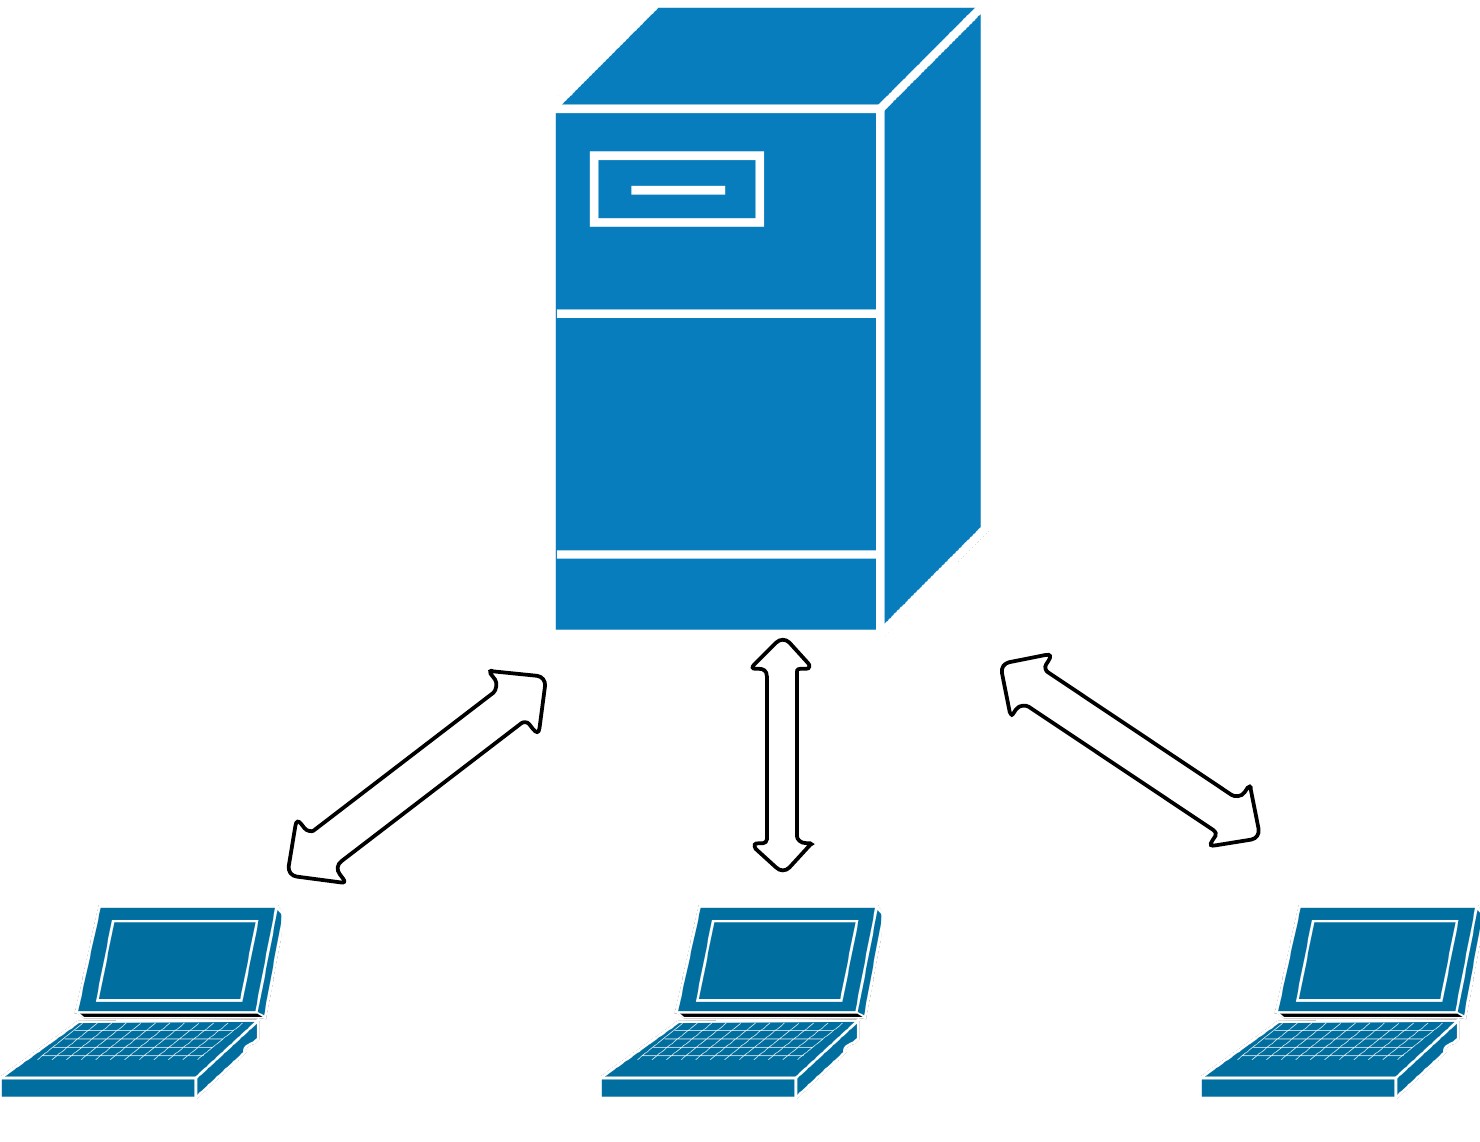
\includegraphics[scale=0.175]{centralized.png}
        \end{center}
    \end{figure}
\end{frame}

\begin{frame}
    \frametitle{Distributed paradigm (Git, Mercurial)}
    \begin{figure}[h!]
        \begin{center}
            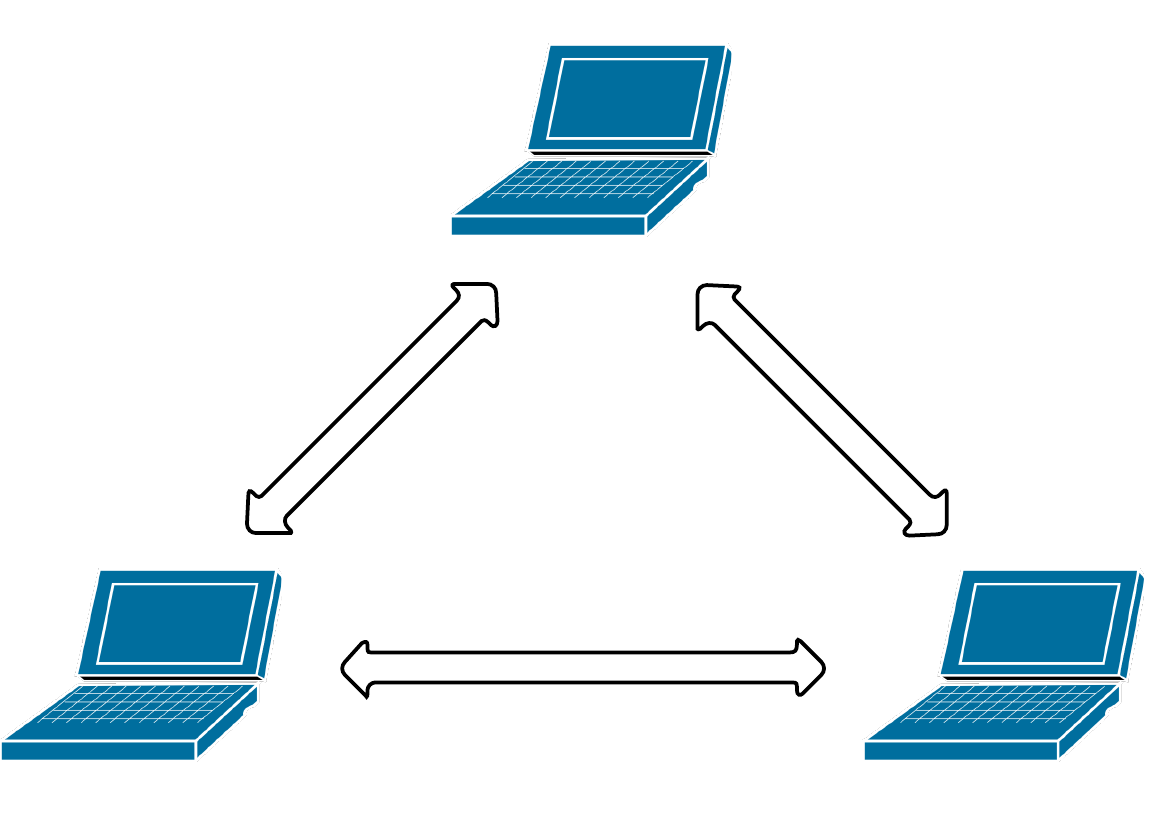
\includegraphics[scale=0.55]{distributed.png}
        \end{center}
    \end{figure}
\end{frame}

\section{Commands}
\begin{frame}
    \frametitle{Git commands}
    \tableofcontents[Commands]
\end{frame}

\begin{frame}
    \frametitle{Git commands}
    \begin{figure}[h!]
        \begin{center}
            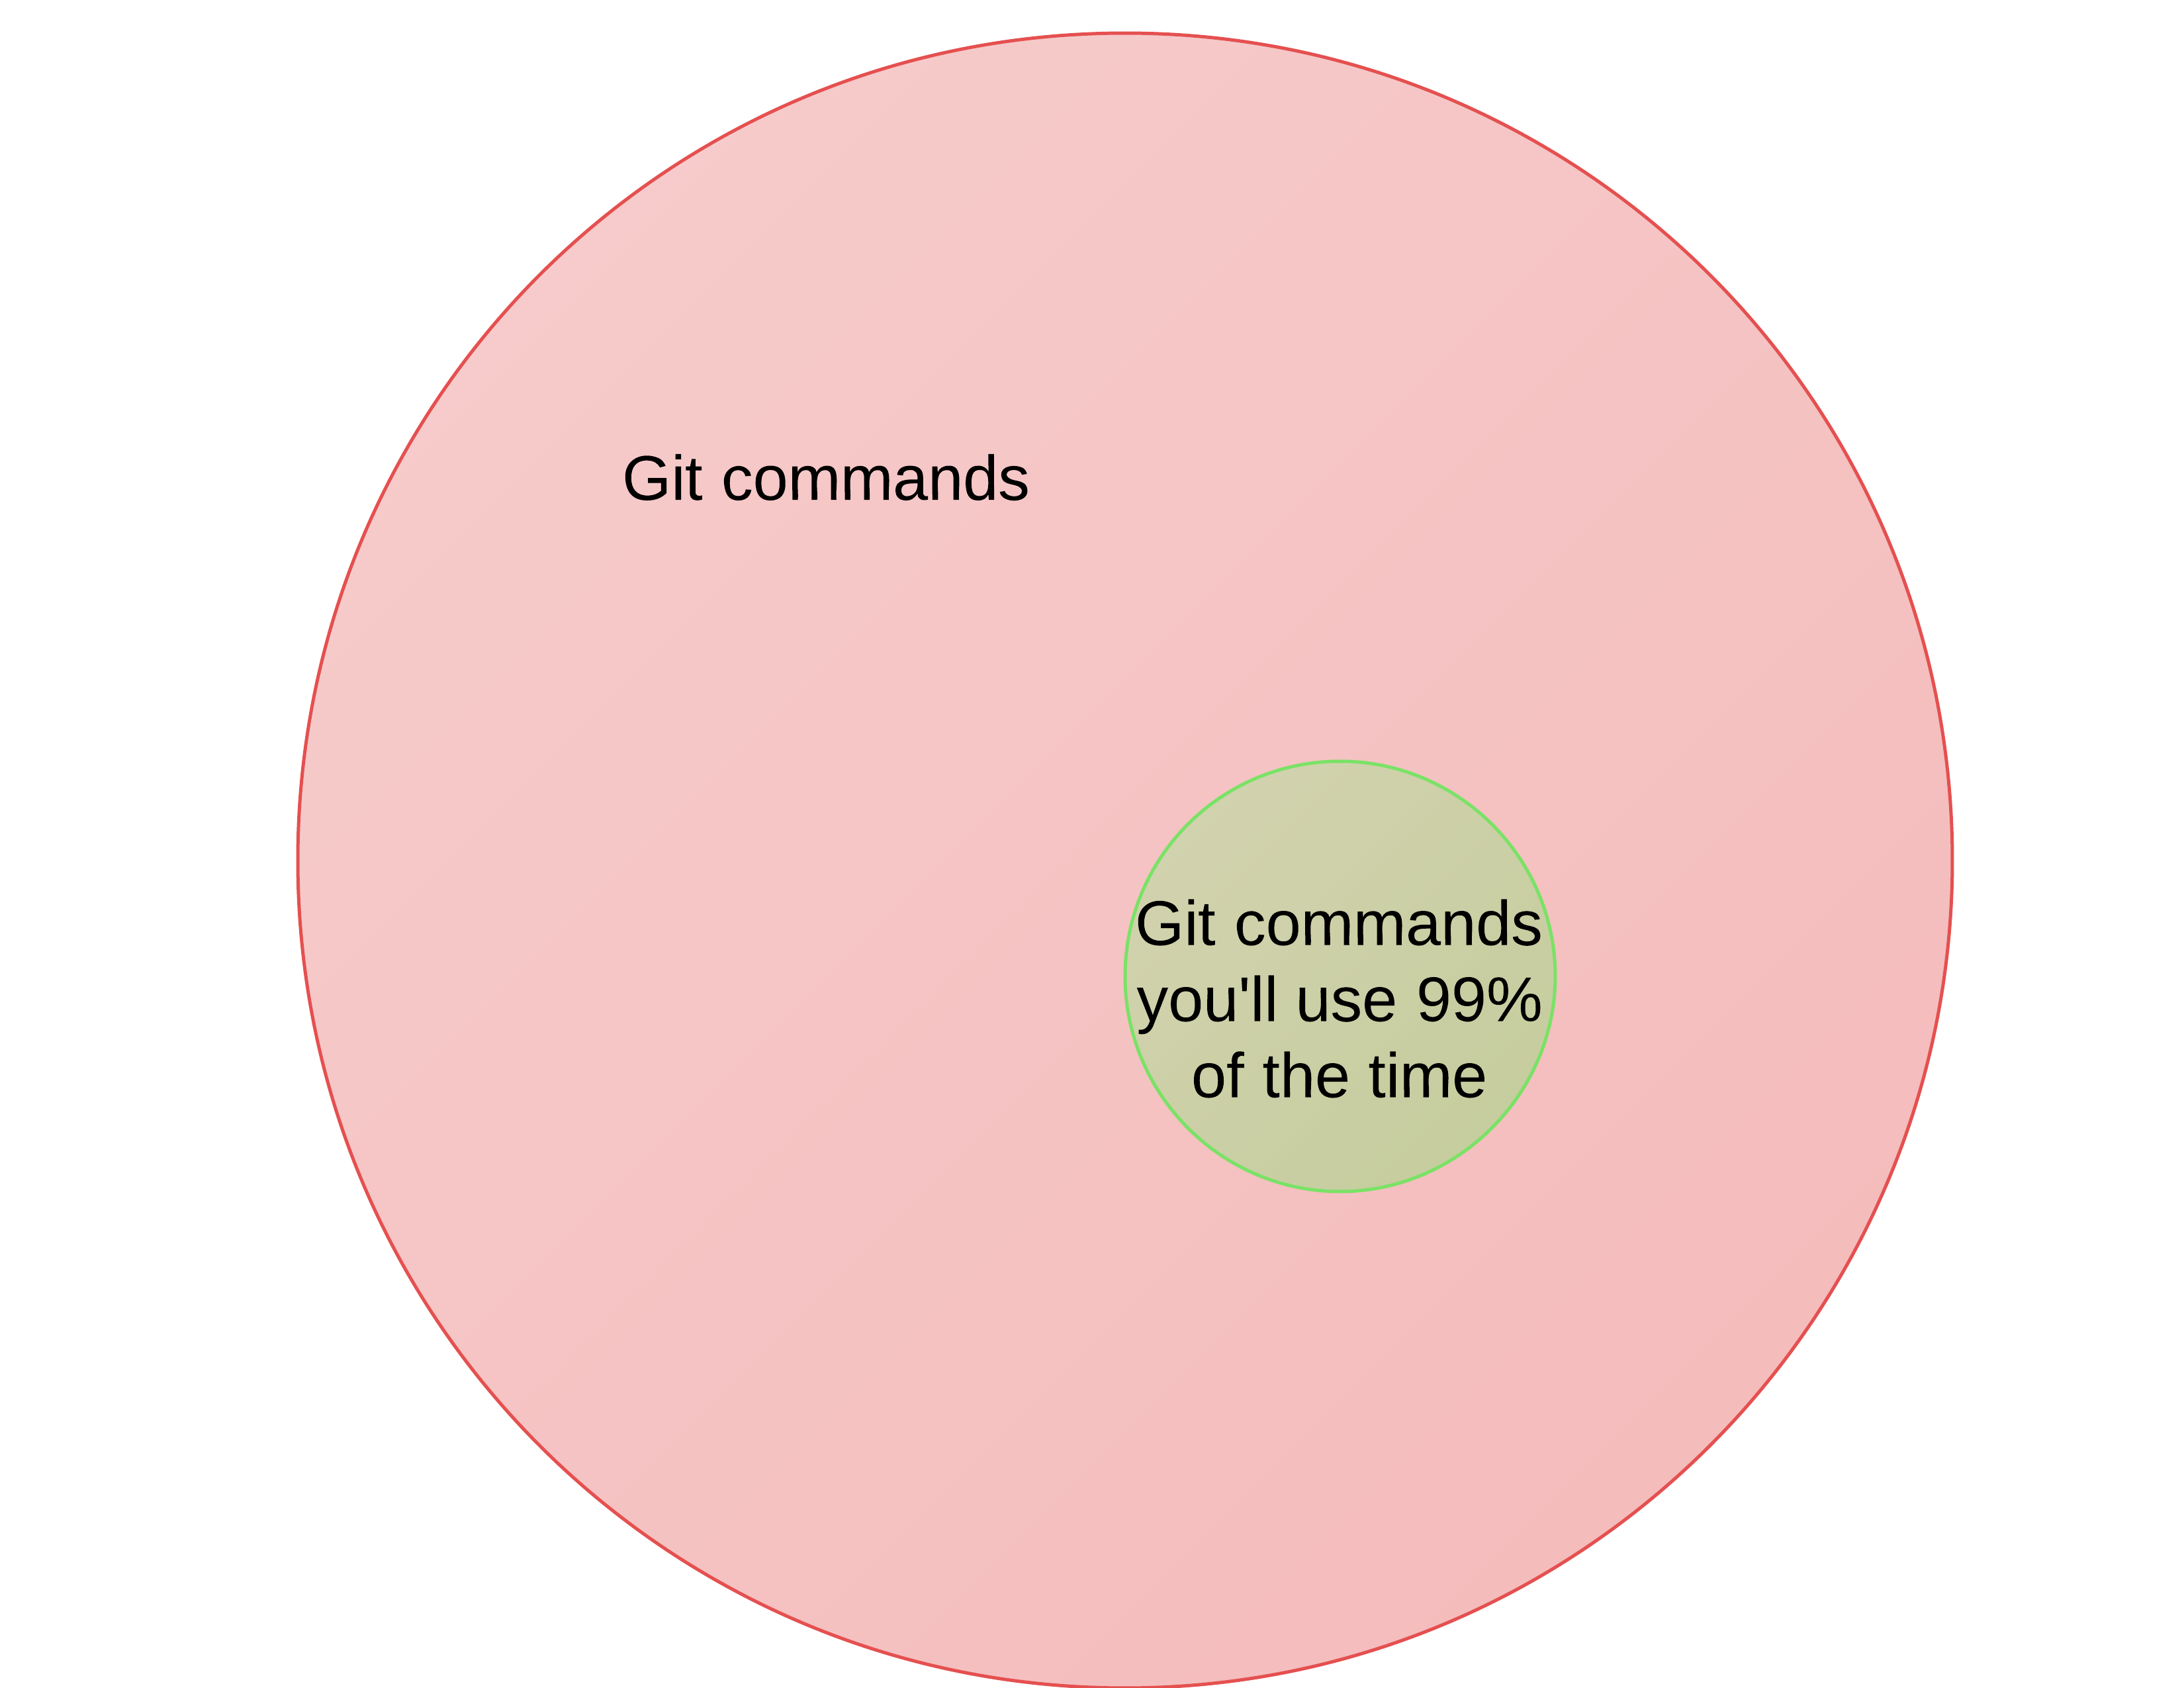
\includegraphics[scale=0.09]{git_commands1.png}
        \end{center} \end{figure}
\end{frame}

\begin{frame}
    \frametitle{Git commands}
    \begin{figure}[h!]
        \begin{center}
            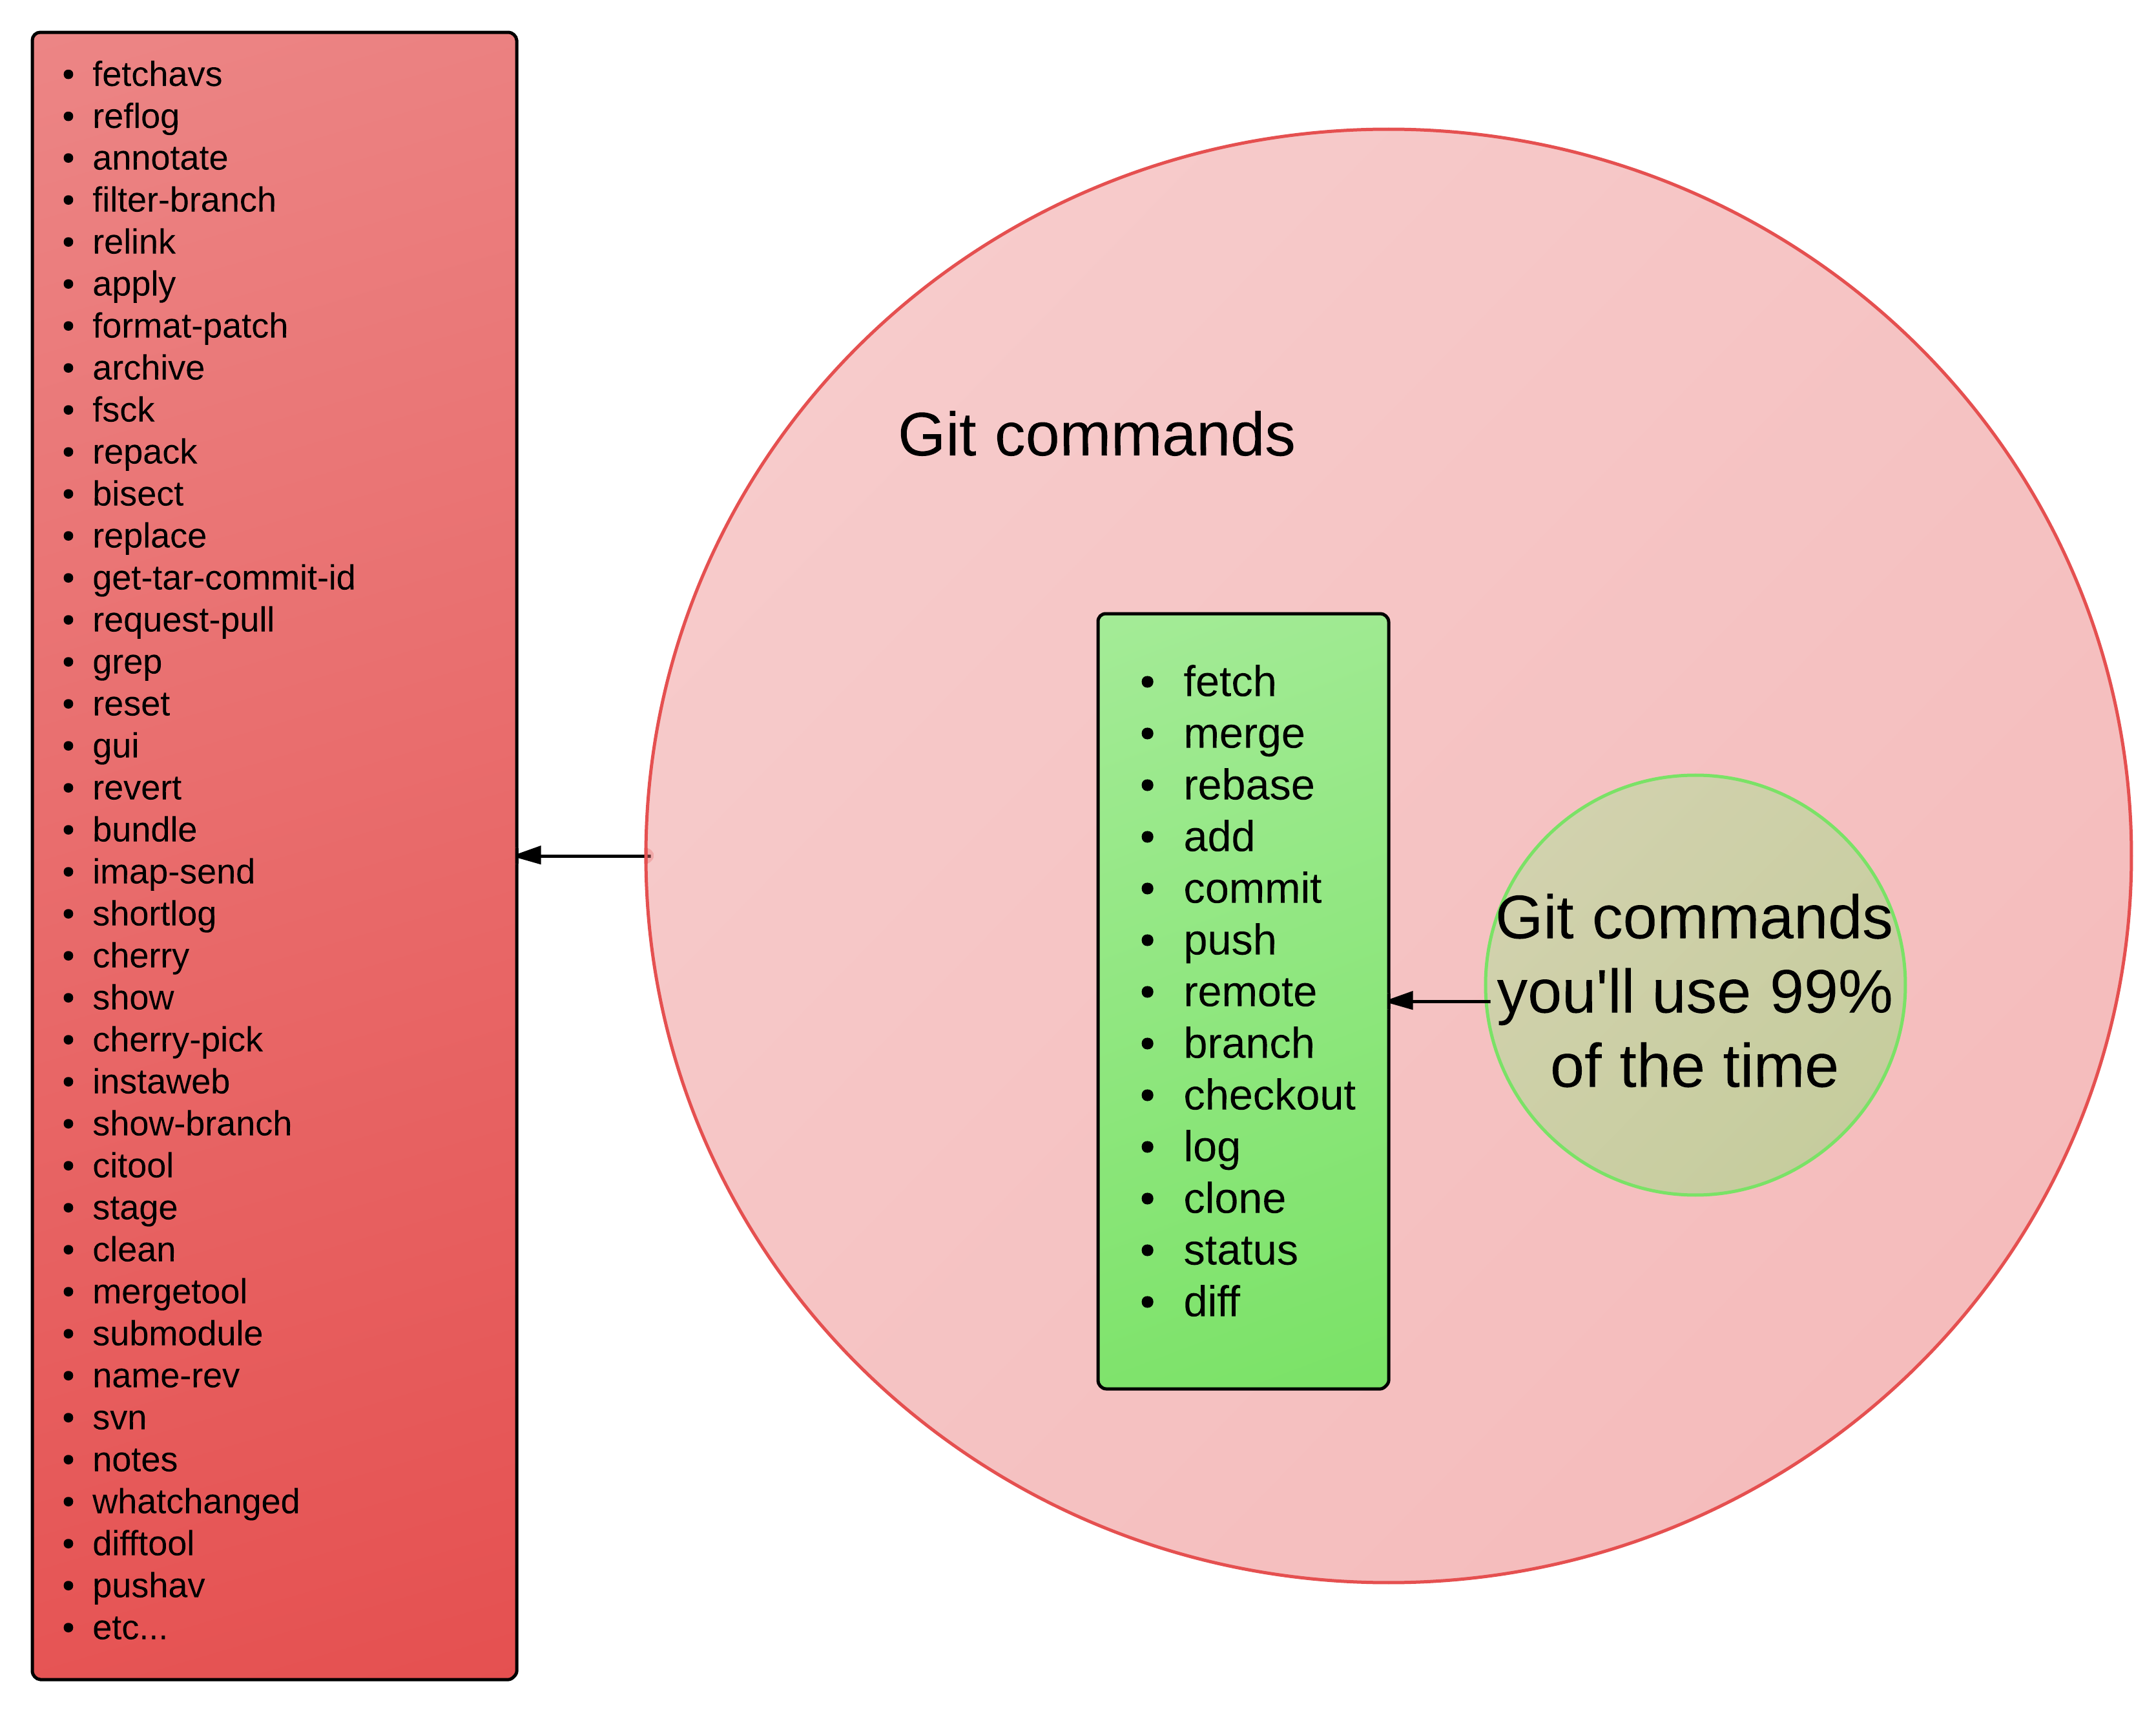
\includegraphics[scale=0.09]{git_commands2.png}
        \end{center}
    \end{figure}
\end{frame}

\begin{frame}
    \frametitle{Git commands}
    \begin{figure}[h!]
        \begin{center}
            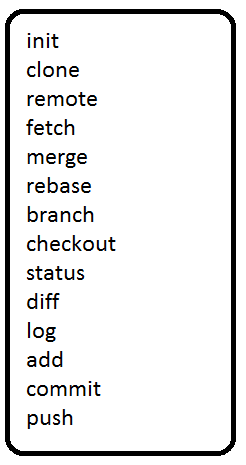
\includegraphics[scale=0.6]{commands.png}
        \end{center}
    \end{figure}
\end{frame}

\begin{frame}
    \frametitle{\$ git init}
    \begin{figure}[h!]
        \begin{center}
            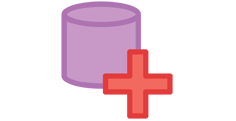
\includegraphics[scale=0.8]{init.png}
        \end{center}
    \end{figure}
\end{frame}

\begin{frame}
    \frametitle{\$ git clone}
    \begin{figure}[h!]
        \begin{center}
            
\includegraphics[scale=0.8]{clone.png}
        \end{center}
    \end{figure}
\end{frame}

\begin{frame}
    \frametitle{\$ git remote}
    \begin{figure}[h!]
        \begin{center}
            
\includegraphics[scale=0.8]{remote.png}
        \end{center}
    \end{figure}
\end{frame}

\begin{frame}
    \frametitle{\$ git fetch}
    \begin{figure}[h!]
        \begin{center}
            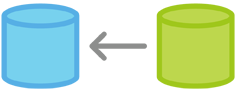
\includegraphics[scale=0.8]{pull.png}
        \end{center}
    \end{figure}
\end{frame}

\begin{frame}
    \frametitle{\$ git merge}
    \begin{figure}[h!]
        \begin{center}
            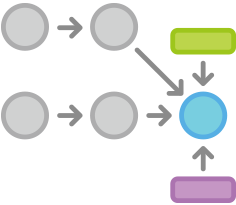
\includegraphics[scale=0.8]{merge.png}
        \end{center}
    \end{figure}
\end{frame}

\begin{frame}
    \frametitle{\$ git rebase}
    \begin{figure}[h!]
        \begin{center}
            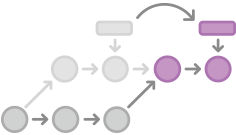
\includegraphics[scale=1.1]{rebase.png}
        \end{center}
    \end{figure}
\end{frame}

\begin{frame}
    \frametitle{\$ git branch}
    \begin{figure}[h!]
        \begin{center}
            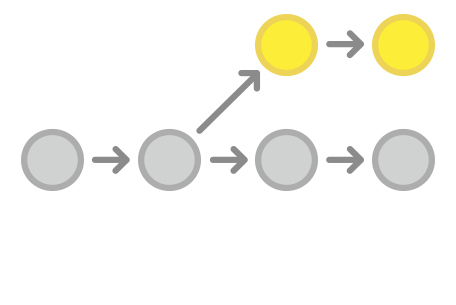
\includegraphics[scale=0.5]{branch.png}
        \end{center}
    \end{figure}
\end{frame}

\begin{frame}
    \frametitle{\$ git checkout}
    \begin{figure}[h!]
        \begin{center}
            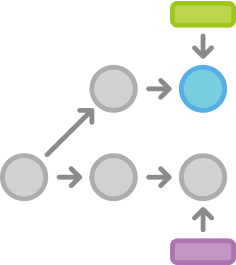
\includegraphics[scale=0.7]{checkout.png}
        \end{center}
    \end{figure}
\end{frame}

\begin{frame}
    \frametitle{\$ git status}
    \begin{figure}[h!]
        \begin{center}
            
\includegraphics[scale=0.8]{status.png}
        \end{center}
    \end{figure}
\end{frame}

\begin{frame}
    \frametitle{\$ git diff}
    \begin{figure}[h!]
        \begin{center}
            
\includegraphics[scale=1.2]{diff.png}
        \end{center}
    \end{figure}
\end{frame}

\begin{frame}
    \frametitle{\$ git log}
    \begin{figure}[h!]
        \begin{center}
            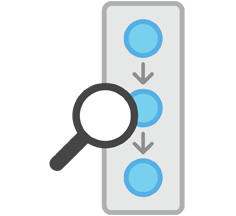
\includegraphics[scale=0.8]{log.png}
        \end{center}
    \end{figure}
\end{frame}

\begin{frame}
    \frametitle{\$ git add}
    \begin{figure}[h!]
        \begin{center}
            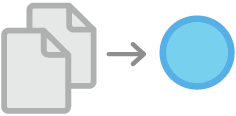
\includegraphics[scale=0.8]{add.png}
        \end{center}
    \end{figure}
\end{frame}

\begin{frame}
    \frametitle{\$ git commit}
    \begin{figure}[h!]
        \begin{center}
            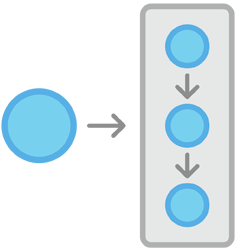
\includegraphics[scale=0.8]{commit.png}
        \end{center}
    \end{figure}
\end{frame}

\begin{frame}
    \frametitle{\$ git push}
    \begin{figure}[h!]
        \begin{center}
            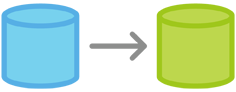
\includegraphics[scale=0.8]{push.png}
        \end{center}
    \end{figure}
\end{frame}

\section{IDEs}

\begin{frame}
    \frametitle{Git commands}
    \begin{figure}[h!]
        \begin{center}
            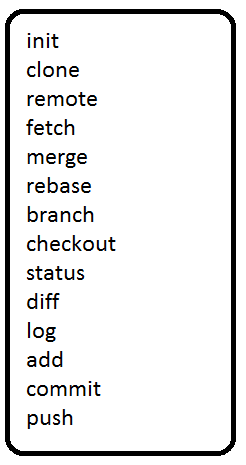
\includegraphics[scale=0.6]{commands.png}
        \end{center}
    \end{figure}
\end{frame}

\begin{frame}
    \frametitle{Eclipse}
    \begin{figure}[h!]
        \begin{center}
            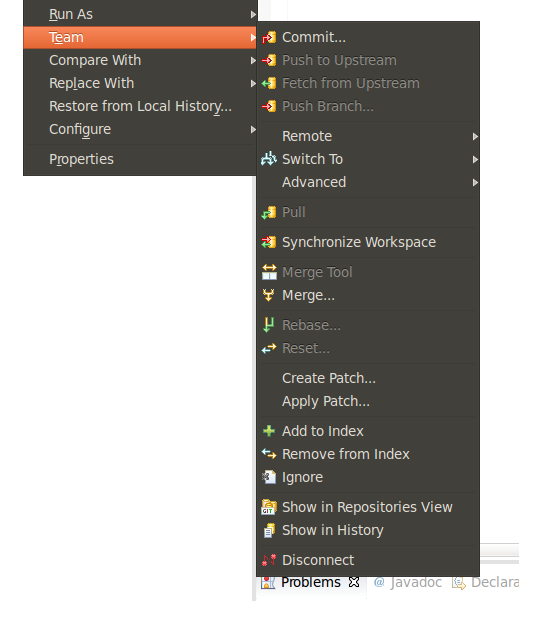
\includegraphics[scale=0.55]{eclipse1.png}
        \end{center}
    \end{figure}
\end{frame}

\begin{frame}
    \frametitle{Eclipse}
    \begin{figure}[h!]
        \begin{center}
            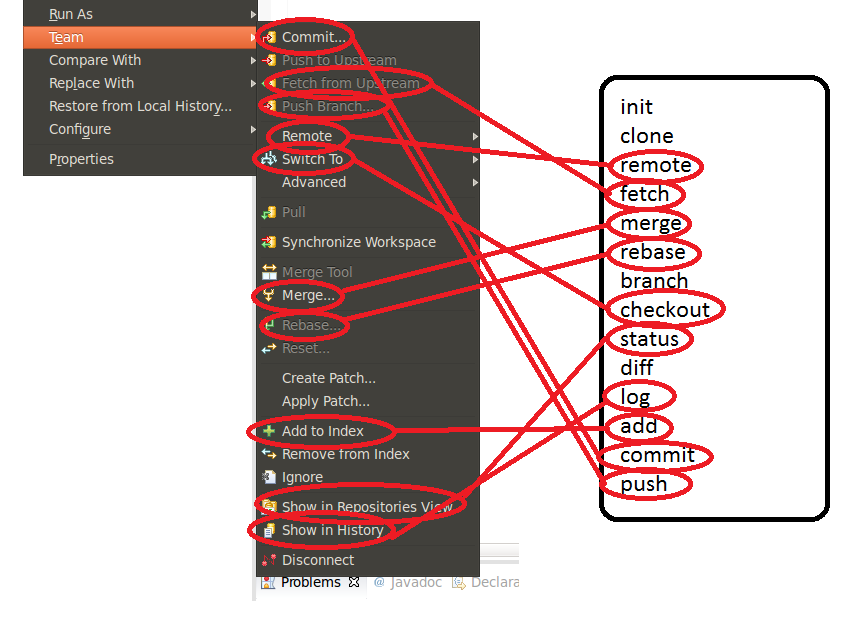
\includegraphics[scale=0.5]{eclipse2.png}
        \end{center}
    \end{figure}
\end{frame}

\begin{frame}
    \frametitle{IntelliJ}
    \begin{figure}[h!]
        \begin{center}
            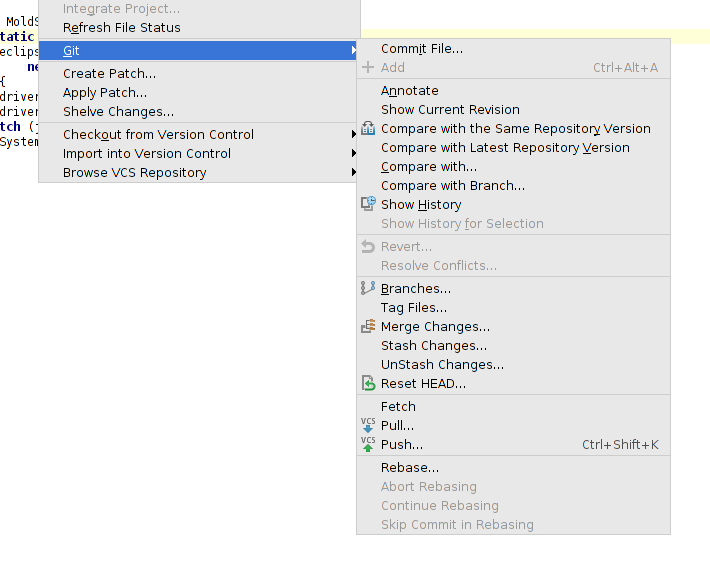
\includegraphics[scale=0.55]{intellij1.png}
        \end{center}
    \end{figure}
\end{frame}

\begin{frame}
    \frametitle{IntelliJ}
    \begin{figure}[h!]
        \begin{center}
            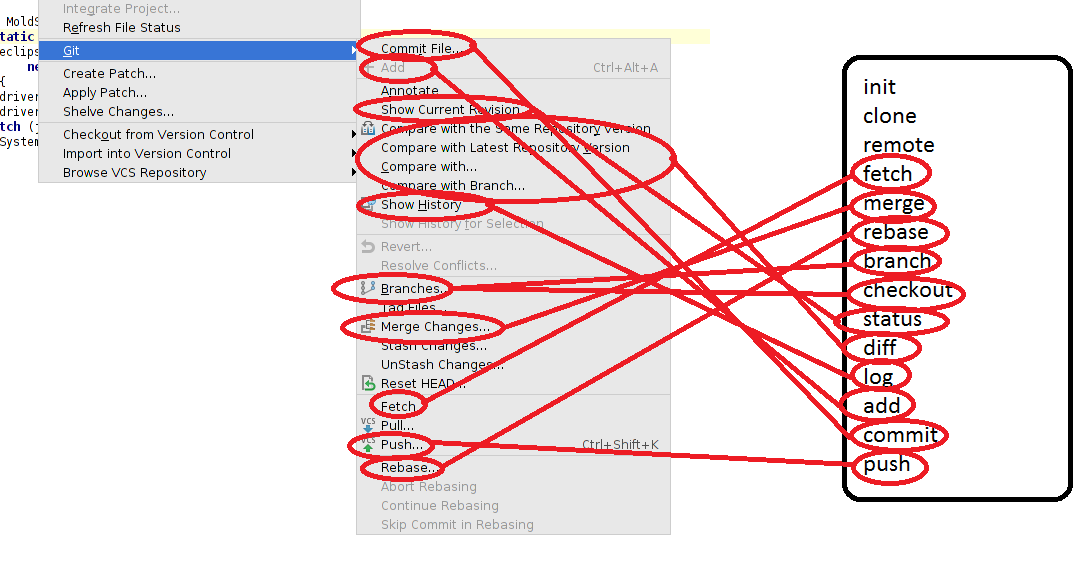
\includegraphics[scale=0.4]{intellij2.png}
        \end{center}
    \end{figure}
\end{frame}

\section{Workflow}

\section{Ressources}

\begin{frame}
    \frametitle{Ressources}
    \begin{center}
        Atlassian has a great straightforward tutorial at
        \url{https://www.atlassian.com/git/}
    \end{center}
\end{frame}

\section{Homework}

\end{document}

